% !TEX root = ../thesis.tex

\chapter{Pravdepodobnostný model kvantového výpočtu - návrh a realizácia}

Cieľom je vytvoriť v jazyku Haskell model, ktorý by dokázal merať stavy
kvantových bitov aj bez ich kolabovania. Na rozdiel od IBM Quantum
Experience tento model môže realizovať unitárne operácie aj paralelne.

\begin{figure}
	\centering 
	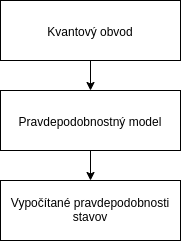
\includegraphics[width=.2\textwidth]{figures/navrh.png} 
	\caption{Konceptuálny návrh programu}
    \label{navrh}
\end{figure}


Pri pohľade na jednoduchý konceptuálny model (obrázok \ref{navrh}) je zrejmé
čo cheme dosiahnuť. Na vstupe je očakávaný kvantový obvod. Samotný program
prebehne tímnto obvodom ako interpreter a zároveň pomerá stavy na daných
miestach v obvode. Nakoniec vypíše výstup v zrozumiteľnej podobe.

\section{Definícia vstupu}

Celý kvantový obvod je možné rozdeliť do vertikálnych blokov alebo levelov.
Každý level obsahuje hradlá, ktorých počet je maximálne rovný počtu 
kvantových bitov, s ktorými daný obvod pracuje. Ak v danom levely nechceme
aplikovať žiadnu operáciu nad bitom, môžme definovať prázdny element.

Čiže kvantový obvod môžeme definovať ako list levelov, pričom level je datová
štruktúra, ktorá obsahuje list hradiel. Okrem hradiel každý level bude
obsahovať prepínač, ktorý siganlizuje či má nastať meranie po aktivácií 
hradiel v leveli.
